\newpage
\subsubsection{Drehräder-Modell}
\begin{figure}[h!]
	\centering
	\begin{subfigure}{.4\textwidth}
		\centering
		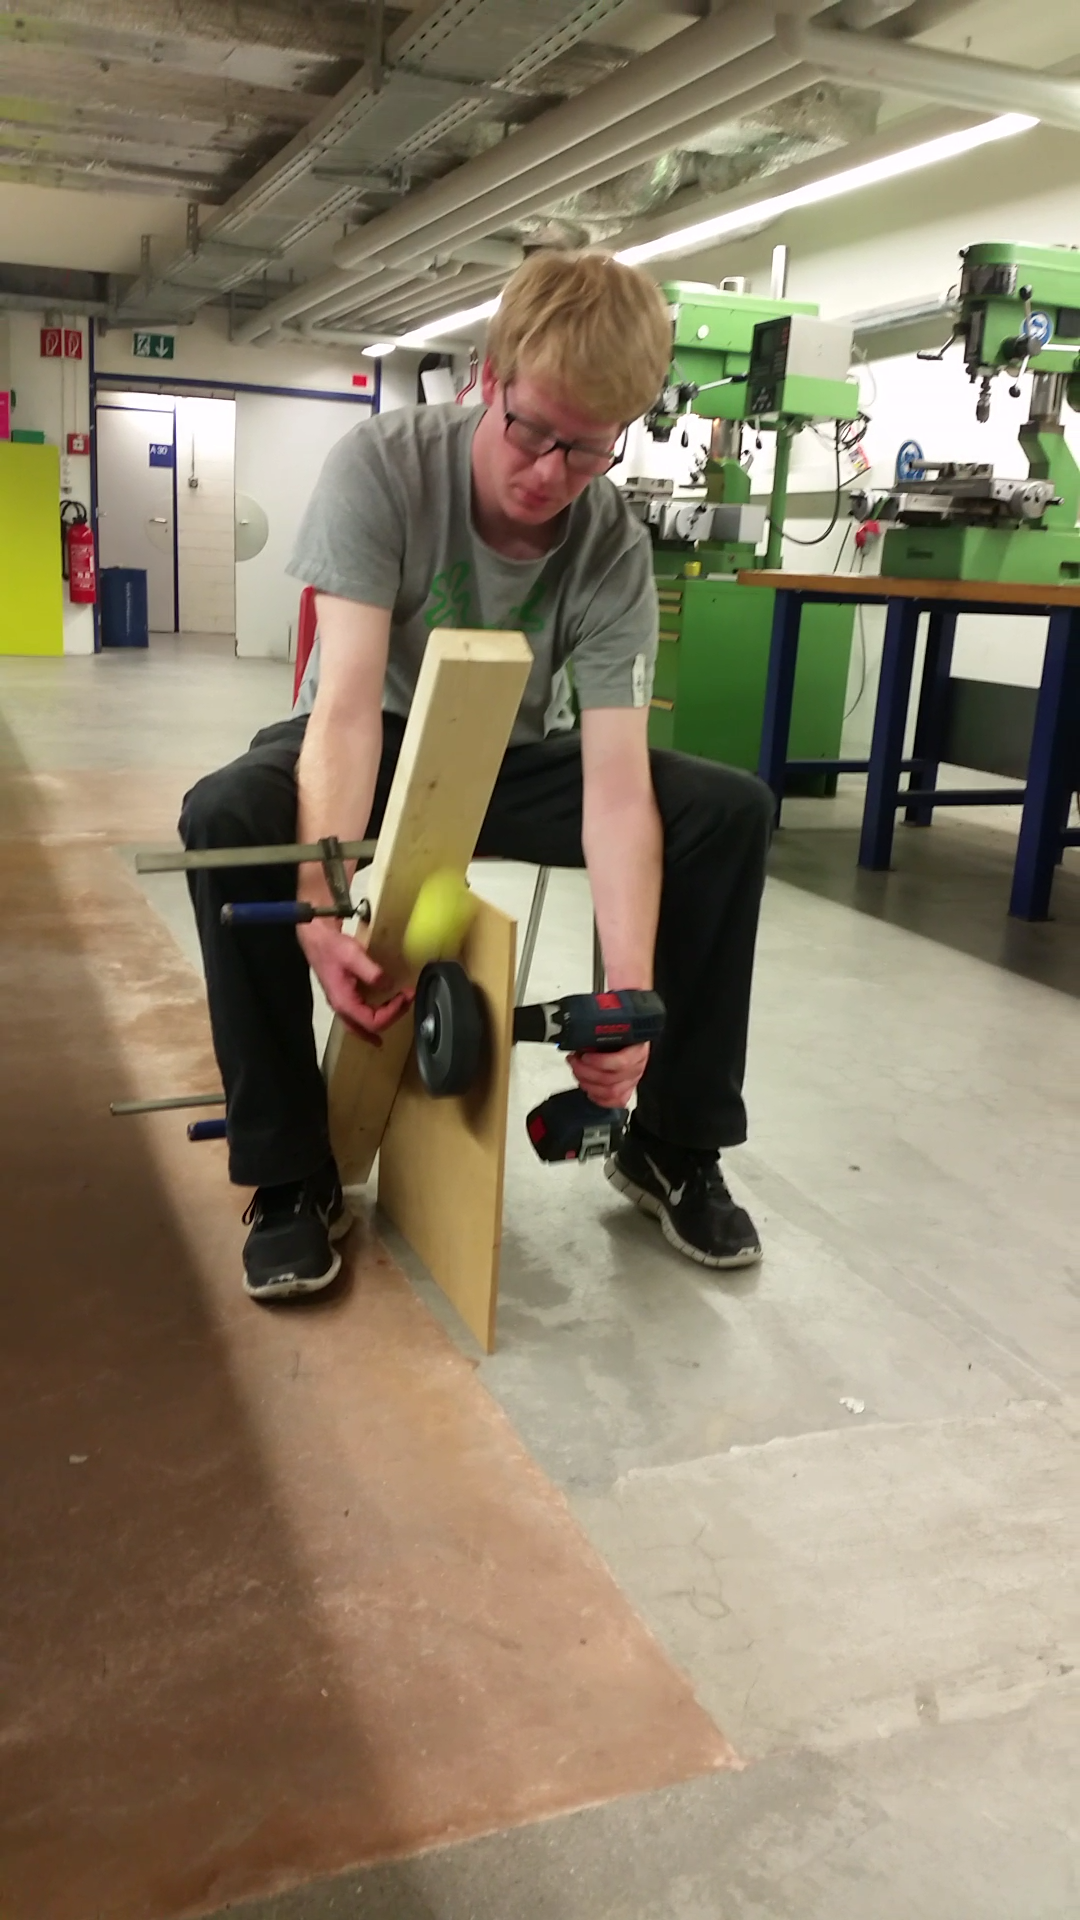
\includegraphics[width=0.6\textwidth]{../../fig/Versuch_Drehrad.png}
		\caption{Schrägen Wurf von der Seite}
		\label{fig:Aufbau der Versuch}
	\end{subfigure} %
	\begin{subfigure}{.4\textwidth}
		\centering
		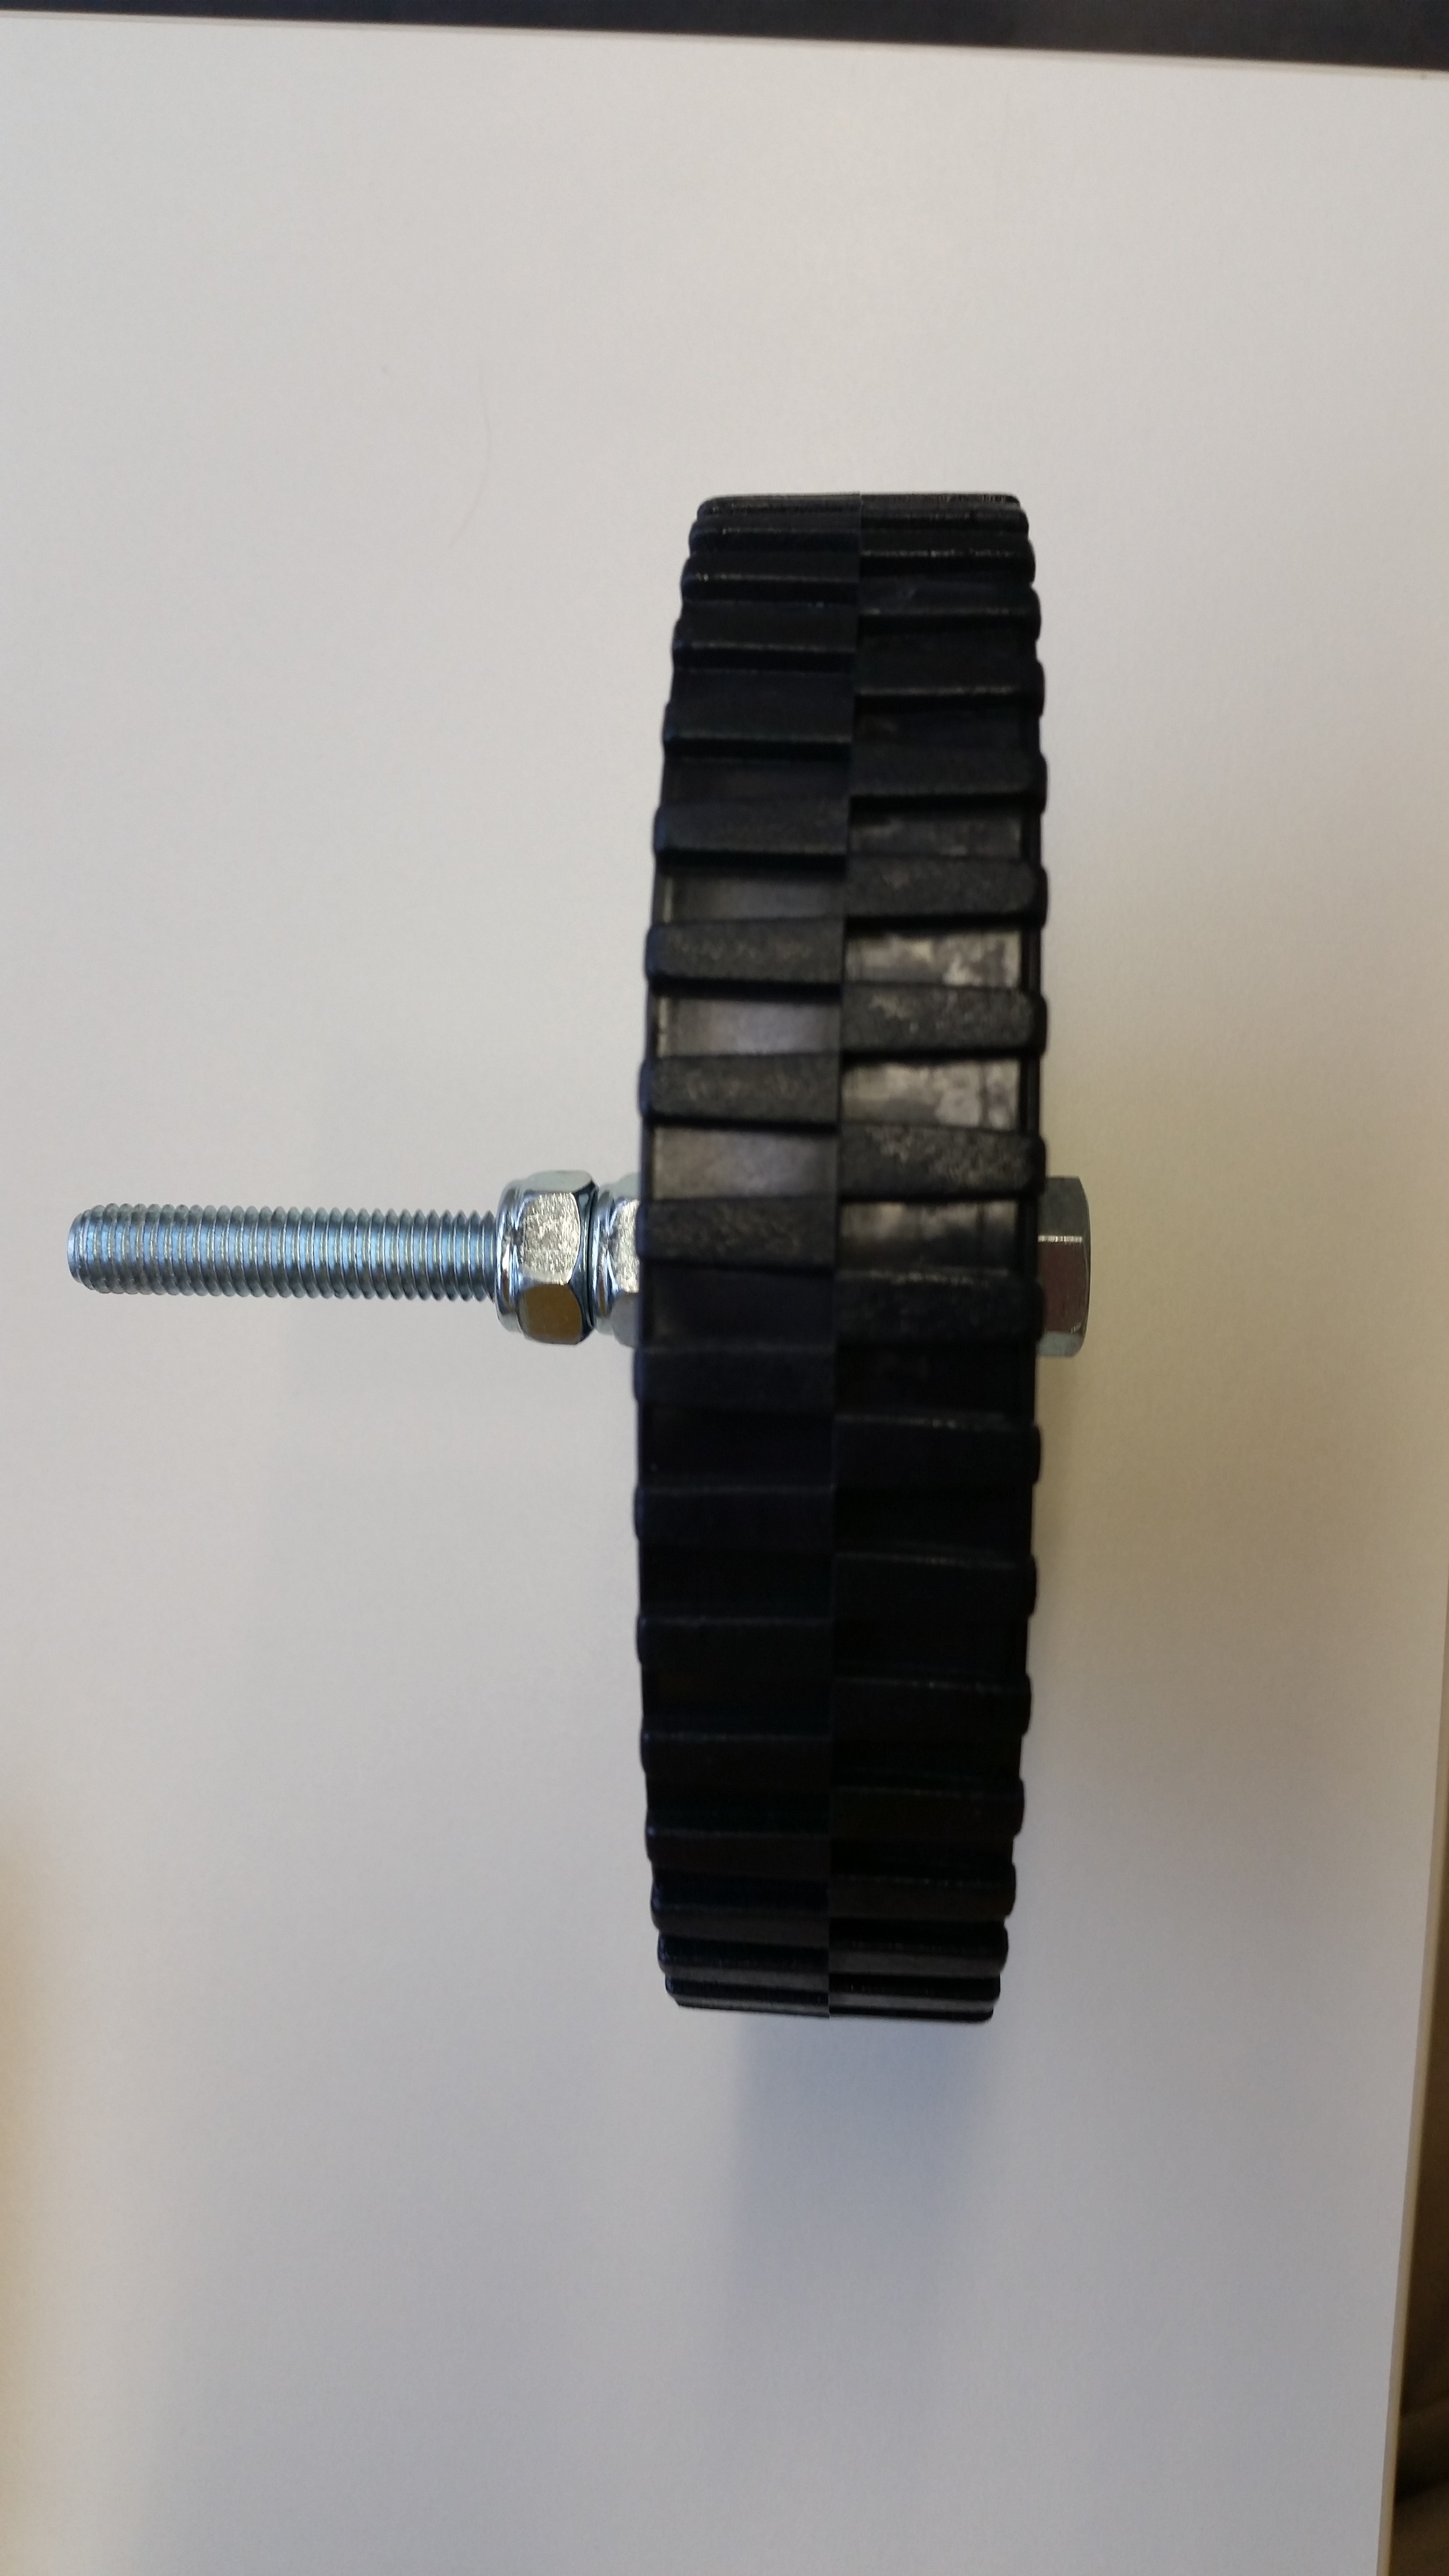
\includegraphics[width=0.6\textwidth]{../../fig/Drehrad_1.jpg}
		\caption{Schrägen Wurf von Oben}
		\label{fig:Drehrad}
	\end{subfigure}
	\caption{Berechnung der Schräger Wurf}
	\label{Drehrad Versuch}
\end{figure}
Mit diesem Versuch sollte festgestellt werden, von welcher Seite (Ober/ Unterseite) her, der Ball beschleunigt werden soll. Zudem sollte der Einfluss vom Drall ermittelt werden. Wir haben einen Polypropylen Rad mit einem Durchmesser von 15cm. verwendet. Als Antrieb wurde eine Akkubohrmaschine eingesetzt. Bei diesem Versuchsaufbau spielte die erreichte Wurfdistanz eine untergeordnete Rolle. Viel wichtiger war die Treffgenaugkeit.  
Der Versuch wurde auf zwei verschiedene Arten durchgeführt: ein erstes mal mit dem Drehrad oberhalb des Balles, und ein zweites Mal mit dem Drehrad auf der Unterseite. Mit diesen unterschiedlichen Versuchsaufbauarten konnte die Auswirkungen auf die Treffgenaugkeit und die Flugbahn bestimmt werden.\\ \\
Nach mehrere Versuche wurde festgelegt, dass beide Varianten recht zuverlässig funktionieren. Da der Prototyp relativ instabil war, haben wir mit schlechteren Ergebnissen gerechnet. Die Bälle erreichten eine Distanz von ca. 1.3 Meter und landeten innerhalb von einem von einem Kreis mit einem Durchmesser von 30cm. 
\\Weiter wurde festgestellt, dass der Wurf mit dem Drehrad auf der Unterseite etwas präziser ist. Der Versuchsaufbau hat ergeben, dass der Drall keinen signifikanten Einfluss auf die Flugbahn hat.\\

